% ****** Start of file apssamp.tex ******
%
%   This file is part of the APS files in the REVTeX 4.2 distribution.
%   Version 4.2a of REVTeX, December 2014
%
%   Copyright (c) 2014 The American Physical Society.
%
%   See the REVTeX 4 README file for restrictions and more information.
%
% TeX'ing this file requires that you have AMS-LaTeX 2.0 installed
% as well as the rest of the prerequisites for REVTeX 4.2
%
% See the REVTeX 4 README file
% It also requires running BibTeX. The commands are as follows:
%
%  1)  latex apssamp.tex
%  2)  bibtex apssamp
%  3)  latex apssamp.tex
%  4)  latex apssamp.tex
%
\documentclass[%
 reprint,
%superscriptaddress,
%groupedaddress,
%unsortedaddress,
%runinaddress,
%frontmatterverbose, 
%preprint,
%preprintnumbers,
%nofootinbib,
%nobibnotes,
%bibnotes,
 amsmath,amssymb,
 aps,
%pra,
%prb,
%rmp,
%prstab,
%prstper,
%floatfix,
]{revtex4-2}
\usepackage{kotex}
\usepackage{physics}
\usepackage{graphicx}% Include figure files
\usepackage{dcolumn}% Align table columns on decimal point
\usepackage{bm}% bold math
%\usepackage{hyperref}% add hypertext capabilities
%\usepackage[mathlines]{lineno}% Enable numbering of text and display math
%\linenumbers\relax % Commence numbering lines

%\usepackage[showframe,%Uncomment any one of the following lines to test 
%%scale=0.7, marginratio={1:1, 2:3}, ignoreall,% default settings
%%text={7in,10in},centering,
%%margin=1.5in,
%%total={6.5in,8.75in}, top=1.2in, left=0.9in, includefoot,
%%height=10in,a5paper,hmargin={3cm,0.8in},
%]{geometry}

\def\rcurs{{\mbox{$\resizebox{.16in}{.08in}{
\includegraphics{ScriptR}}$}}}
\def\brcurs{{\mbox{$\resizebox{.16in}{.08in}{
\includegraphics{BoldR}}$}}}
\def\hrcurs{{\mbox{$\hat \brcurs$}}}

\begin{document}


\title{프랑크-헤르츠 실험 보고서}

\author{서울대학교 전기정보공학부 2018-12432 박정현}
 \email{alexist@snu.ac.kr}
\date{실험일자 : 11.13.2023}% It is always \today, today,
             %  but any date may be explicitly specified

\begin{abstract}
본 실험에서는 Ne을 용수철 모델로 근사하여 absorption cross section을 계산하고 Child-Langmuir law에 따라 cathod, anode 사이에 흐르는 전류를 보정하여 인가된 전압에 따른 전류를 이론적으로 예측하였다. 또한 역전압에 따른 효과를 이론적으로 확인하여 모델의 타당성을 확인하였다. 계산된 모델을 통해 energy level과 decay rate를 측정하였으며 기존의 이론치와 비교한 후 그 이유에 대해 논의한 뒤 정확한 energy level과 decay rate를 측정하는 방법을 제시하였다.
\end{abstract}

%\keywords{Suggested keywords}%Use showkeys class option if keyword
                              %display desired
\maketitle

%\tableofcontents

\section{Introudction}
에너지의 양자화는 현대물리의 가장 중요한 원리이다. 특히 원자의 에너지가 양자화되어 있음을 보인 것은 매우 중요한 일이다. 독일의 물리학자 프랑크와 헤르츠는 1914년 원자 기체에 전기장을 가하여 전류값을 측정하여 내부 에너지가 양자화 되어 있음을 보였다. 본 실험에서는 플랑크, 헤르츠가 수행했던 실험을 재현하고 이를 통해 원자 내부의 에너지가 양자화 되어 있음을 간접적으로 증명하고 열전자, 원자의 에너지에 대한 이해도를 높인다.

\subsection{Ne 에너지 레벨}
Ne의 에너지 레벨은 Fig.\ref{fig:Neenergy}와 같다.[1] 19eV이상의 에너지를 가진 전자와 충돌하게 되면 3s, 3p와 같은 state로 1s,2s, 혹은 2p level의 전자가 excite하게 된다. 3s$\rightarrow$3p, 3s$\rightarrow$2p, 2s$\rightarrow$2p 혹은 2p$\rightarrow$1s으로의 전이가 발생하게 된다.

\begin{figure}[htbp]
	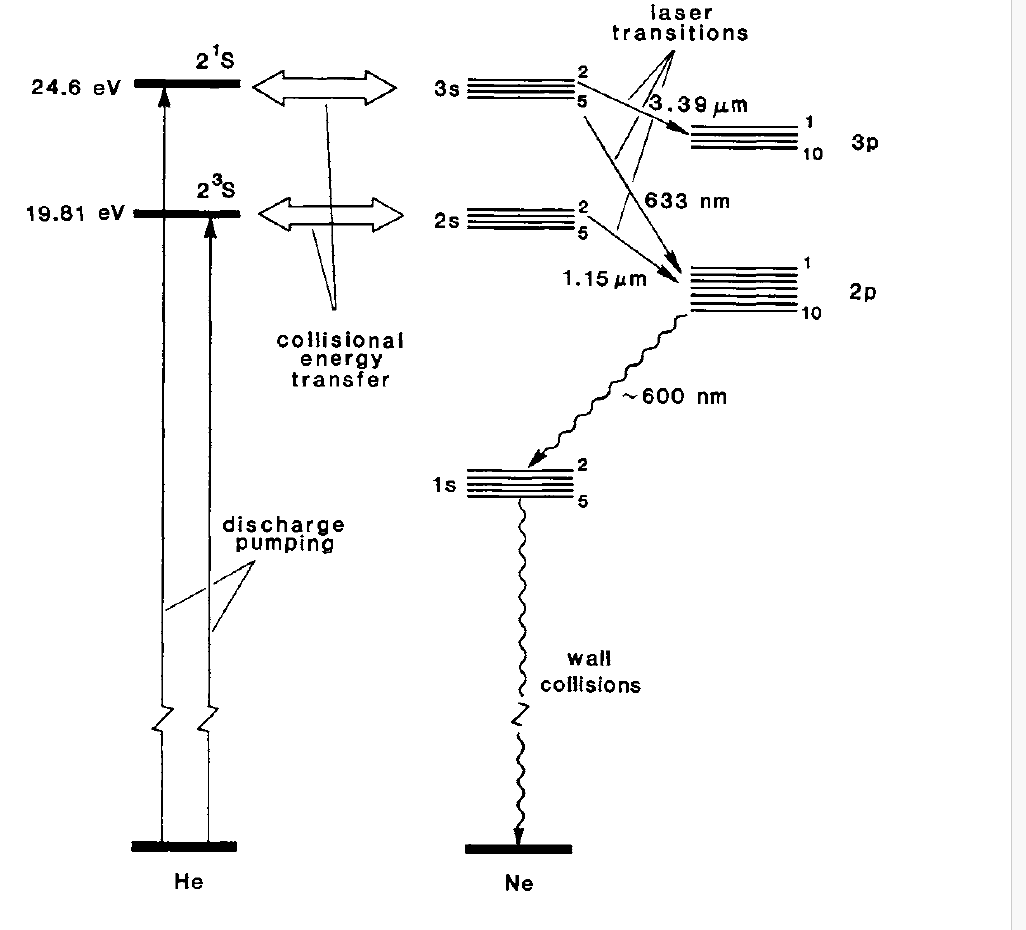
\includegraphics[width = 0.85\linewidth]{Neenergy.png}% Here is how to import EPS art
	\caption{\label{fig:Neenergy}Ne 원자 에너지 레벨}
\end{figure}

원자의 전자를 용수철 상수로 근사하여도 어느정도의 광학적 성질을 분석하는데 큰 문제가 발생하지 않는다.[3] $\omega$의 주파수를 가진 전기장 내에서 이때 전자의 운동은 아래와 같이 풀어 낼 수 있다.
\begin{align}
	m(\ddot{\vec{x}}+\Gamma_{0}\dot{\vec{x}} + \omega_{0}^{2}\vec{x}) &= e\vec{E}_{0}\exp(-i\omega t)
\end{align}
가속하는 전자가 방출하는 power는 아래와 같은 방법을 통해 계산할 수 있다.
\begin{align}
	P &= \frac{e^{2}}{6\pi\varepsilon_{0}c^{3}}\frac{1}{2}\Re[\ddot{x}\ddot{x}^{*}]\\
	&= \frac{e^{4}\omega^{4}}{6\pi\varepsilon_{0}^{2}c^{4}m^{2}} \frac{I_{0}}{(\omega_{0}^{2}-\omega^{2})^{2}+\Gamma_{0}^{2}\omega^{2}}
\end{align}
$I_{0}$는 입사하는 전자기파의 에너지이고 $\Gamma_{0}$는 spontaneous decay rate에 해당한다. Spontaneous decay rate는 아래와 같이 계산된다.[5]

\begin{align}
	\Gamma_{0} &= \frac{e^{2}\omega_{0}^{2}}{6\pi \epsilon_{0}mc^{2}}\\
	&= \frac{e^{4}V_{0}^{2}}{6\pi \hbar^{2}\epsilon_{0}mc^{2}} \label{eq:theorydecay}
\end{align}

따라서 전자의 scattering cross section은 아래와 같다.
\begin{align}
	\sigma_{sc} &= \frac{e^{4}\omega^{4}}{6\pi\varepsilon_{0}^{2}c^{4}m^{2}} \frac{1}{(\omega_{0}^{2}-\omega^{2})^{2}+\Gamma_{0}^{2}\omega^{2}}
\end{align}

일반적으로 전기감수율은 아래의 식을 만족한다. 
\begin{align}
	\exp[-\Im \chi \omega x /c ] &= \exp(-n\sigma_{abs}x)
\end{align}

전기장에 의해 생성된 전기 쌍극자 모멘트는 용수철에 전자가 매달린 모델을 이용하면 아래의 식을 만족함을 알 수 있다.

\begin{align}
	\vec{P} &= ne\vec{x}\\
	&= \frac{ne^{2}/m}{\omega^{2}-i\Gamma_{t}+\omega_{0}^{2}}
\end{align}

둘 사이의 관계식을 통해 아래의 식이 성립함을 알 수 있다. 단, 여기서 $\Gamma_{t}$는 non-radiative decay와 같이 spontaneous decay rate 외의 모든 decay factor를 합친 decay rate에 해당한다. 
\begin{align}
	\Im \chi &= \frac{ne^{2}}{m\epsilon_{0}} \frac{\Gamma_{t}\omega}{(\omega^{2}-\omega_{0}^{2})^{2} + \Gamma_{t}\omega^{2}}
\end{align}

앞서 계산한 결과들을 바탕으로 아래의 식이 성립함을 알 수 있다.
\begin{align}
	\sigma_{abs} &\simeq 6\pi (c/\omega_{0})^{2}\Bigg(\frac{\Gamma_{t}}{\Gamma_{0}}\Bigg)\frac{(\Gamma_{0}/2)^{2}}{(\omega-\omega_{0})^{2}+(\Gamma_{t}/2)^{2}}
\end{align}

앞서 계산한 식은 전자기파에 대해서 풀은 식이지만 고전적인 영역에서 광자가 아닌 전자를 통해 에너지가 전달된다는 analogy를 이용하면 앞서 계산한 cross section을 사용해도 무방할 것이다. 즉, $eV = \hbar \omega$로 두어 전자의 에너지를 $\omega$로 대응시켜 식을 사용할 수 있다. 열전자들이 가속되어 Ne gas주변에 시간에 따라 일정한 수의 전자가 존재하는 경우 전류는 아래와 같은 Child-Langmuir법칙에 따라 흐르게 된다. [2]

\begin{align}
	J &= KV^{3/2}/d^{2}
\end{align}

하지만 전자와 Ne 원자가 충돌하는 경우 전자의 운동 에너지는 Ne원자의 전자로 전달되고 전자는 더 작아진 운동에너지를 가지고 scattering하게 된다.  따라서 Ne가스와 충돌하는 기체들이 존재하는 경우 해당 전자들은 에너지를 잃은 속도로 anode에 도달하게 되므로 전류량은 감소하게 될 것이다. 총 N개의 Ne 원자가 단면적 A의 관에 존재하는 경우 전체 전자들중 충돌하는 비율을 $\eta$라고 했을 때 $\eta$는 아래의 식을 만족한다.

\begin{align}
	\eta &= \frac{N\sigma_{abs}}{A}
\end{align}

전자가 Ne원자를 excite시킬 만큼 충분한 에너지를 가지게 되는 위치를 $d_{0}$라고 할 때 $d_{0}$부터 다시 가속하게 되고 이러한 전자가 $d_{0}$에서 $d$까지 random하게 위치한다고 가정하면 감소하는 전류량은 아래의 식을 만족하면서 감소하게 된다. 단, $\omega \simeq \omega_{0}$ 주변에서의 적분값만 충분히 큰 값을 가지므로 $\eta$ 를 적분 밖으로 꺼내고 $d_{0}\simeq d$로 근사한다.

\begin{align}
	\Delta J &= -\frac{1}{d-d_{0}}\int_{d_{0}}^{d} \eta KV^{3/2}(1-\frac{x}{d})^{3/2}/(d-x)^{2}dx\\
	&\simeq -\frac{NKV^{3/2}}{Ad^{2}} 6\pi \Bigg(\frac{c}{\omega_{0}}\Bigg)^{2}\Bigg(\frac{\Gamma_{t}}{\Gamma_{0}}\Bigg)\frac{(\Gamma_{0}/2)^{2}}{(\omega-\omega_{0})^{2}+(\Gamma_{t}/2)^{2}}
\end{align}


따라서 $\hbar \omega = eV$로 두는 경우 총 전류는 아래와 같이 나타난다.

\begin{align}
	&\begin{aligned}
	J_{tot} &= \frac{KV^{3/2}}{d^{2}}\Bigg(1 -\frac{N 6\pi}{A} \Bigg(\frac{c}{\omega_{0}}\Bigg)^{2}\Bigg(\frac{\Gamma_{t}}{\Gamma_{0}}\Bigg)\\
	&\frac{(\hbar\Gamma_{0}/2e)^{2}}{(\hbar\omega/e-\hbar\omega_{0}/e)^{2}+(\hbar\Gamma_{t}/2e)^{2}}\Bigg)
	\end{aligned}\\
	&\simeq KV^{3/2}/d^{2}\left(1-\frac{\beta}{(V-V_{0})^{2}+\gamma^{2}} \right)
\end{align}

단, $\gamma$와 $\beta$는 아래의 식을 만족한다.

\begin{align}
	\beta &= N\frac{ 6\pi}{A} \Bigg(\frac{c}{\omega_{0}}\Bigg)^{2}\Bigg(\frac{\Gamma_{t}}{\Gamma_{0}}\Bigg) (\hbar\Gamma_{0}/2e)^{2} \\
	\gamma &= \hbar\Gamma_{t}/2e 
\end{align}

따라서 위의 식으로부터 vally의 FWHM은 아래와 같이 계산할 수 있다.

\begin{align}
	FWHM &= 2\gamma\\
	&= \hbar\Gamma_{t}/e 
\end{align}

따라서 FWHM을 측정하면 해당 원자의 decay rate를 측정할 수 있다. 전자가 여러번 충돌하는 경우 주파수 $\omega - \omega_{0}$에 대해서 동일한 논리가 적용이 될 것이다. 따라서 아래의 식을 만족한다. $\beta_{1} = 0.01$, $\beta_{2} = 0.02$, $\beta_{3} = 0.03$, $\gamma_{1} = 0.01$, $\gamma_{2} = 0.02$, $\gamma_{3} = 0.03$, K=1, d=1 을 대입하여 계산한 이론적인 전류값은 Fig.\ref{fig:SIM}와 같다.

\begin{align}
	\begin{aligned}
	J_{tot} &= KV^{3/2}/d^{2}\Bigg(1-\frac{\beta_{1}}{(V-V_{0})^{2}+\gamma_{1}^{2}} \\
	&-\frac{\beta_{2}}{(V-2V_{0})^{2}+\gamma_{2}^{2}} -\frac{\beta_{3}}{(V-3V_{0})^{2}+\gamma_{3}^{2}} \cdots \Bigg)
	\end{aligned}
\end{align}

\begin{figure}[htbp]
	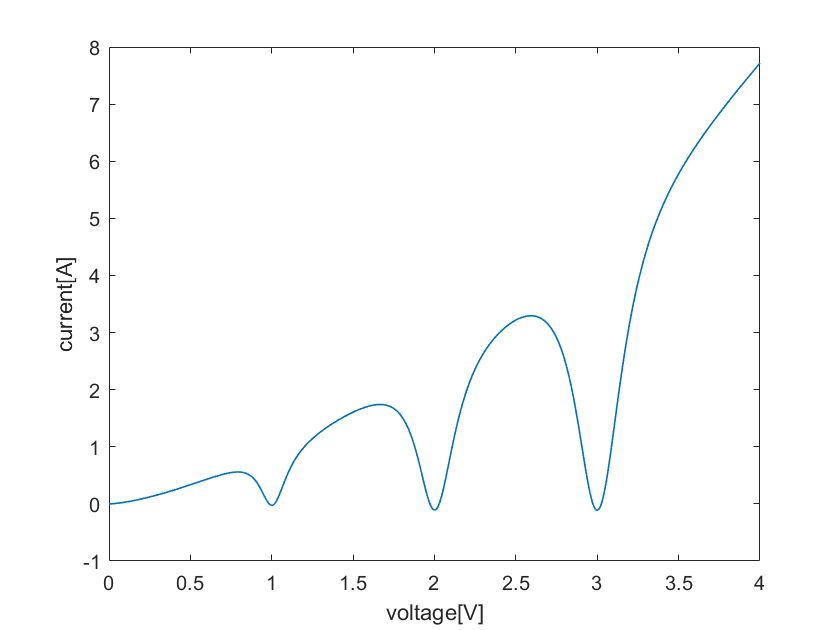
\includegraphics[width = 0.85\linewidth]{SIM.png}% Here is how to import EPS art
	\caption{\label{fig:SIM}Voltage vs Current 이론적 예측}
\end{figure}

따라서 실제 실험 결과에서 Fig.\ref{fig:SIM}와 같이 vally가 발생하는 지점이 주기적인 경우 해당 주기 사이의 에너지를 Ne의 level 사이의 에너지라고 결론지을 수 있으며 $\hbar \omega_{0}$를 측정할 수 있다. 따라서 해당 실험을 통해 decay rate와 Ne 내부의 에너지 간격을 측정할 수 있다.

전자가 cathode에 도달하기 직전에 역전압이 걸려 있는 경우 역전압 영역 직전의 전자들은 $eV$의 에너지를 가질 것이다. 역전압을 $V_{R}$이라고 하는 경우 V가 작은 경우 충분한 양의 전자가 cathode에 도달하지 못할 것이다. 하지만 반대로 V가 충분히 큰 경우 $V_{R}$보다 전압이 커져 anode로 다시 돌아가는 전자는 없을 것이며 근사적으로 양단에 $V-V_{R}$의 전압이 인가된 것과 같은 전류가 흐를 것이다. 이때 V가 $V_{R}$보다 충분히 크므로 이 때의 $V_{R}$은 무시할 수 있을 것이다. 하지만 Ne과 충돌하여 scattering된 전자들은 Ne으로부터 $eV_{0}$만큼의 에너지를 뺏겨 충분한 에너지가 없으므로 역전압에 의해 가속되어 다시 anode로 돌아가게 될 것이다. 따라서 아래와 같은 식을 도출할 수 있다.

\begin{align}
	\begin{aligned}
	J_{tot} &= KV^{3/2}/d^{2}\Bigg(1-\frac{\beta_{1}(1+\alpha_{1}V_{R})}{(V-V_{0})^{2}+\gamma_{1}^{2}} \\
	&-\frac{\beta_{2}(1+\alpha_{2}V_{R})}{(V-2V_{0})^{2}+\gamma_{2}^{2}} -\frac{\beta_{3}(1+\alpha_{3}V_{R})}{(V-3V_{0})^{2}+\gamma_{3}^{2}} \cdots \Bigg)
	\end{aligned}
\end{align}

$V_{R} = 1V$, $\alpha_{i} = 0.01$을 대입하면 Fig.\ref{fig:SIM2}와 같은 결과가 나타난다. 따라서 실제 실험에서 cathod 부근에 역전압을 인가하여 Ne의 scattering에 의한 vally를 좀더 정확하게 확인할 수 있을 것이다.

\begin{figure}[htbp]
	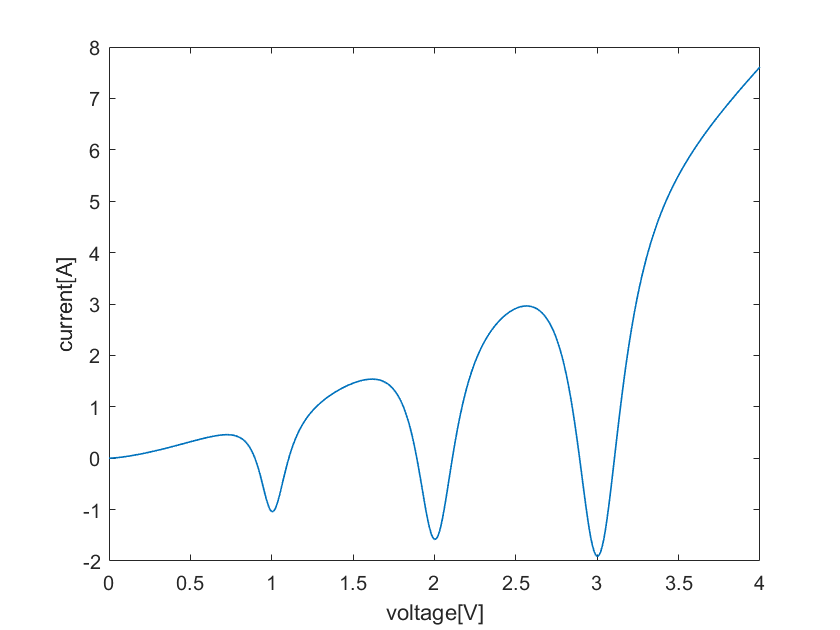
\includegraphics[width = 0.85\linewidth]{SIM2.png}% Here is how to import EPS art
	\caption{\label{fig:SIM2}역전압이 있는 경우 Voltage vs Current 이론적 예측}
\end{figure}

\section{Experimental}
본 실험에서는 3B Scientific 사의 UE502040 프랑크 헤르츠 실험 장비를 이용하였다. 주어진 실험장비의 구조는 Fig.\ref{fig:EXP}와 같다. $U_{F}$는 필라멘트를 가열하여 열전자를 만들고 $U$는 열전자를 가속하는 전압이다. $U_{GA}$는 anode에 도달하는 전자를 감속시키는 역전압에 해당한다. Function generator를 이용해 주기적으로 삼각파를 만들어 oscilloscope을 이용해 측정을 수행한다. 이 때 주기는 second scale에 해당하므로 RF효과는 무시하여도 무방하다.

\begin{figure}[htbp]
	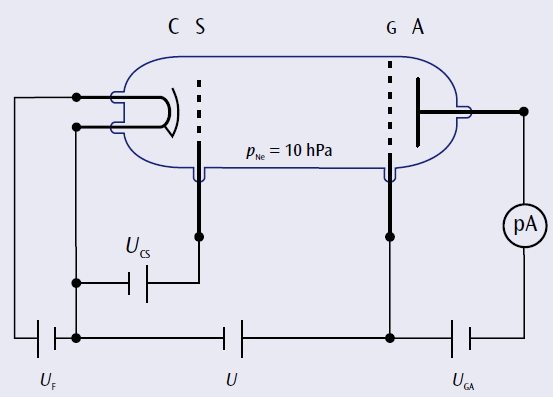
\includegraphics[width = 0.85\linewidth]{EXP.png}% Here is how to import EPS art
	\caption{\label{fig:EXP}프랑크 헤르츠 실험 장비}
\end{figure}

\section{Data \& Results}
아래 Figs.\ref{fig:EXP1}, \ref{fig:EXP2}은 역전압에 따른 실험 측정 결과를 보여준다. 이론적으로 예측한 역전압에 따른 전류값과 동일한 결과를 나타냄을 알 수 있다. 1/10 attenuation을 고려하여 Oscilloscope을 통해 측정된 vally 사이의 간격은 $17.6, 17.6, 20\pm 2 V$이다. 따라서 Ne의 energy level사이의 간격은 $18.4\pm 0.91eV$이며 앞서 Ne의 원자 구조에서 예측한 값과 $10\%$내의 오차에서 일치한다. FWHM은 약 $10\pm2 V$로 이를 통해 계산된 $\Gamma_{t}$는 $(2.42\pm 0.40)\times10^{15}s^{-1}$이다. 따라서 Ne의 $3p$ 오비탈의 life time은 $(4.13\pm0.82)\times 10^{-16}sec$이다. 알려진 바에 따르면 Ne의 $^{3}P_{2}$의 life time은 $14.7sec$이지만 해당 level의 경우 $^{1}S_{0}$ level과 first electric dipole 에서 selection rule을 만족하지 못해 meta stable에 해당하므로 비교하는데 어려움이 있다.[4] $^{1}S - ^{1}P_{0}$ transition의 경우  이론적으로 계산한 수치에 따르면 $2.48\times10^{12}s^{-1}$의 decay rate를 가짐을 알려져 있으며[6] 해당값보다 약 1000배가량 큰 오차를 가진다. 
\begin{figure}[htbp]
	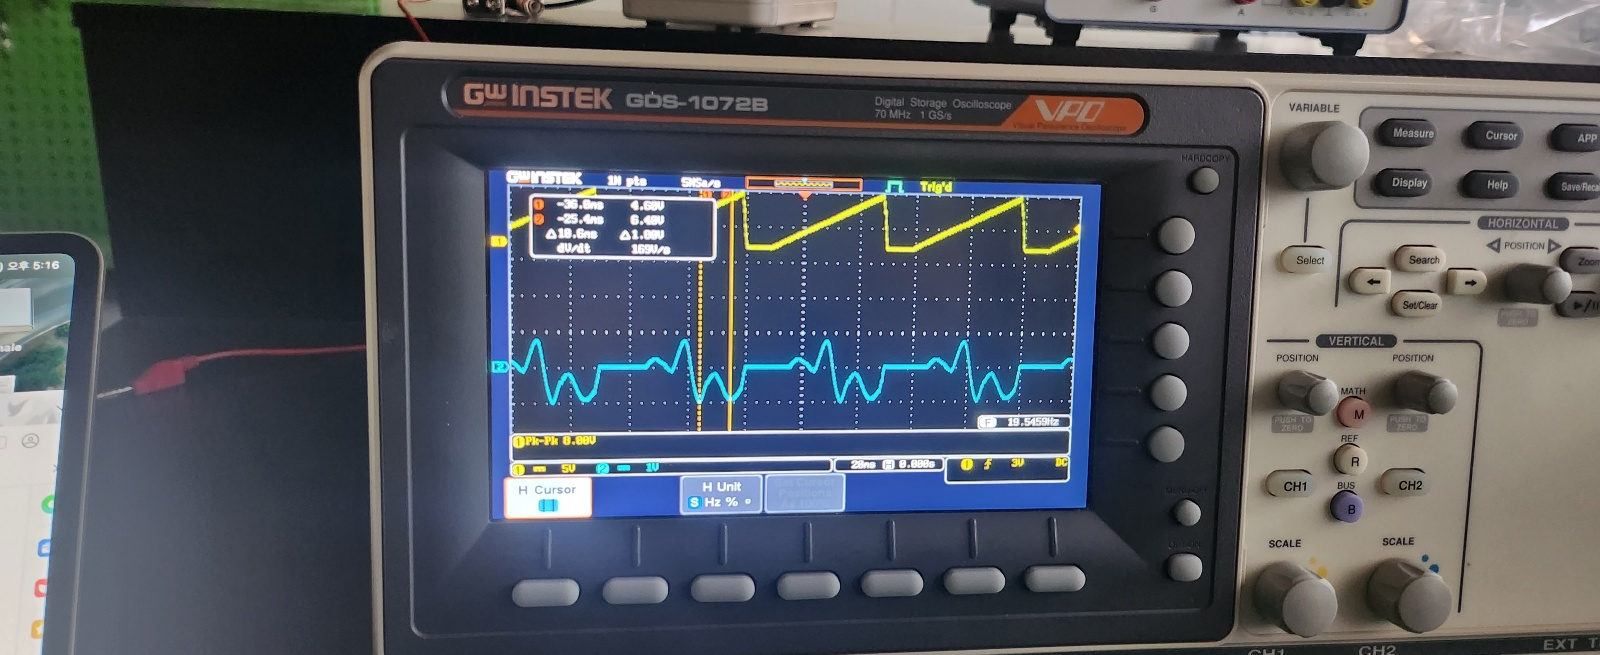
\includegraphics[width = 0.85\linewidth]{EXP1.png}% Here is how to import EPS art
	\caption{\label{fig:EXP1}역전압이 강하게 인가된 경우}
\end{figure}
\begin{figure}[htbp]
	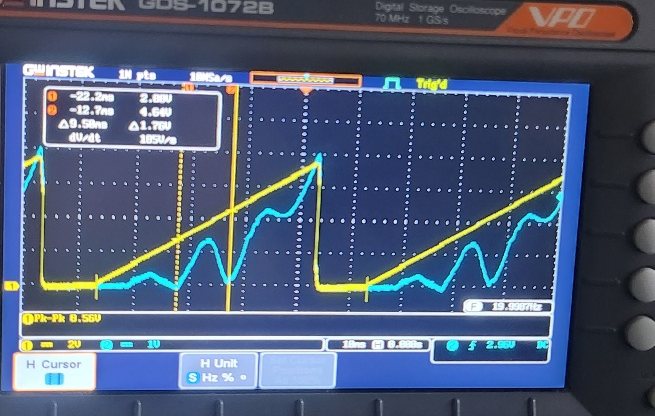
\includegraphics[width = 0.85\linewidth]{EXP2.png}% Here is how to import EPS art
	\caption{\label{fig:EXP2}역전압이 적절히 인가된 경우}
\end{figure}


\section{Conclusion \& Discussions}
본 실험에서 측정한 Ne의 에너지 간격은 이론적인 예측과 잘 일치하였으며 역전압을 인가한 경우, 그렇지 않은 경우 모두 이론적으로 예측한 결과와 동일한 결과를 나타내었다. 따라서 이를 통해 Ne의 내부에너지가 양자화 되어 있음을 간접적으로 증명하였다.

앞서 논의한 모델들을 통해 Ne의 life time을 추산하였으나 이론적인 예측 값과 $1000$배의 오차를 가졌다. 이것은 이전에 수행된 실험[4]의 경우 MOT를 이용해 완전히 외부 열원과 차단된 Ne의 life time을 측정한 것이며 meta stable state의 life time을 측정한 것이므로 본 실험에서 측정한 life time보다 더 긴 값을 가질 것이므로 비교하는데 무리가 있다고 결론지었다. 또한 이론적으로 계산된 decay rate[6]은 모든 level로부터 decay 하는 rate를 계산한 것이 아닌 두 level사이의 decay rate를 계산한 것이며 주변의 열적인 요소들과 non radiative decay rate와 같은 요소들이 모두 무시되었다. 따라서 실험적으로 측정된 decay rate가 더 큰 값을 가지며 앞서 무시된 요소들이 약 1000배 가량의 오차를 만들었다고 결론지었다.

상온에서는 열적인 요동으로 인해 원자들이 운동하게 되면 서로 충돌하면서 braodening이 일어나게 된다. 따라서 프랑크 헤르츠 실험 장비를 이용해 정확한 decay rate를 측정하기 위해서는데 모든 Ne원자들을 저온으로 냉각하여  doppler broadening이 일어나지 않도록 해야 한다. 또한 enviroment의 radiation 또한 모두 차단되어 이로 인한 decay가 발생하지 않도록 해야한다. 이를 통해 더 narrow한 linewidth를 측정할 수 있을 것이고 더 정확한 energy level과 decay rate를 측정할 수 있을 것이다. 또한 충분히 narrow해지는 경우 다른 level로부터의 decay를 모두 구분할 수 있게 되므로 이론적인 예측과 더 정확히 비교할 수 있을 것이다. 또한 oscilloscope을 컴퓨터 데이터로 받아 fitting하는 경우 더 정확한 FWHM을 계산할 수 있을 것이다.

프랑크 헤르츠 실험 장비를 이용하지 않고 정확한 decay rate를 측정하기 위해서는 아래 Fig.\ref{fig:ADVEXP} 와 같은 실험을 통해 측정할 수 있다. Decay rate를 측정하려는 물질을 짧은 시간동안 펄스를 가해 excite를 하고 photo detector에서 감쇠하는 시간을 측정하는 것이다,[7] Energy level의 간격은 rabi oscillation을 하는것이 제일 정확하지만 주어진 실험 장비에서 AOM을 통해 주파수를 바꾸면서 나타나는 peak의 높이에 따라 그래프를 fitting하여 가장 큰 peak를 나타내는 frequency를 energy level 사이의 간격으로 측정할 수 있을 것이다.
\begin{figure}[htbp]
	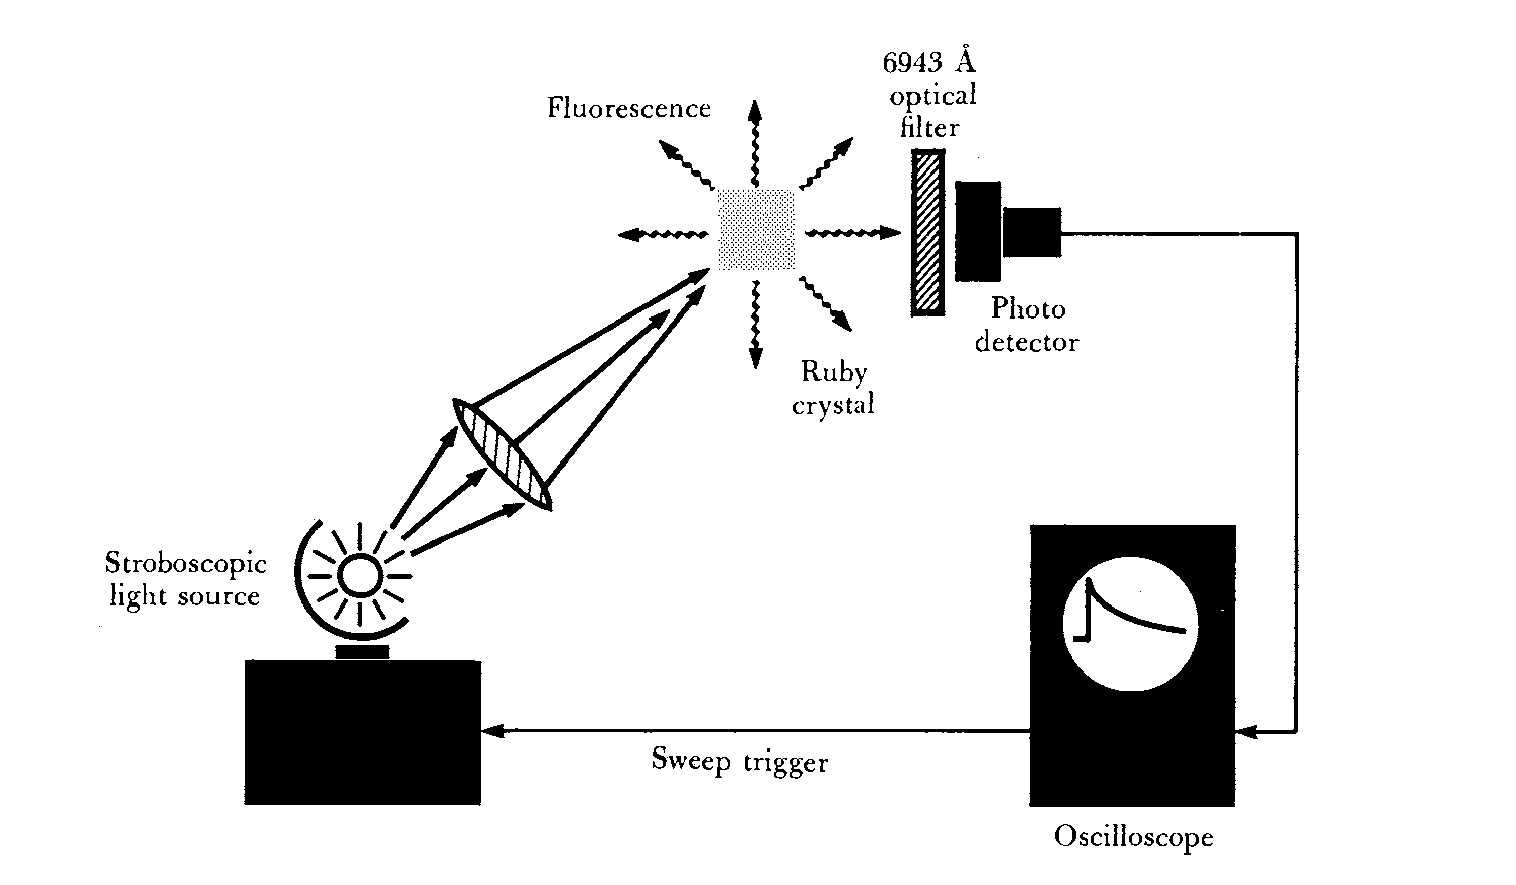
\includegraphics[width = 0.85\linewidth]{ADVEXP.png}% Here is how to import EPS art
	\caption{\label{fig:ADVEXP}Decay rate 측정 장비}
\end{figure}
 

\section{Reference}
[1] Siegman, A. E. (1986, January 1). An Introduction to Lasers. In \textit{Lasers} (1st ed., p. 65). University Science Books.

[2] Griffiths, D. J. (2017, June 29). Electrostatics. In \textit{Introduction to Electrodynamics} (4th ed., p. 109). Cambridge University Press.

[3] 안경원, Laser Physics, 2nd Semester, 2020

[4] Zinner, M., Spoden, P., Kraemer, T., Birkl, G., \& Ertmer, W. (2003, January 30). Precision measurement of the metastable3P2lifetime of neon. \textit{Physical Review A}, 67(1). https://doi.org/10.1103/physreva.67.010501

[5] Griffiths, D. J. (2017, January 1). Quantum Mechanics in Three Dimensions. In \textit{Introduction to Quantum Mechanics}. (pp. 131-154). Cambridge University Press.

[6] Wiese, B. M., Smith, W. L., \& Glennon, M. W. (1966, January 1). \textit{Atomic Transition Probabilities: Vol. 1}: Hydrogen Through Neon (1st ed.). United Stated Department of Commerce. (p. 152)

[7] Siegman, A. E. (1986, January 1). Electric-Dipole Transitions In Real Atoms. In \textit{Lasers} (1st ed., pp. 119–121). University Science Books.
\end{document}
%
% ****** End of file apssamp.tex ******
